\documentclass{mcmthesis}
%[draft]
\mcmsetup{
	CTeX = false,
	tcn = {2504496},
	problem = \textcolor{red}{A},
	sheet = true,
	titleinsheet = true,
	keywordsinsheet = true,
	titlepage = false,
	abstract = false
}
\setlength{\parindent}{2em} % 调整缩进宽度(例如 2em)
\usepackage{tcolorbox}
\usepackage{xcolor}
\usepackage{enumitem}
\usepackage{adjustbox} % 在导言区添加
\definecolor{customblue}{RGB}{165,216,255} % 定义 #a5d8ff 的 RGB 值
\definecolor{deepblue}{RGB}{0,74,173}      % 配套深蓝色

% ================ 环境定义 ================
\newenvironment{featurebox}[1]{%
	\begin{tcolorbox}[
		colback=white,                  % 白色背景
		colframe=customblue,            % 边框颜色 #a5d8ff
		colbacktitle=customblue,        % 标题背景色
		coltitle=deepblue,              % 标题文字颜色
		arc=3mm,                        % 圆角半径
		boxrule=1.5pt,                  % 边框粗细
		title={\large\bfseries #1},     % 标题内容
		fonttitle=\sffamily,            % 无衬线字体
		top=10pt,                       % 上边距
		bottom=10pt,                    % 下边距
		left=10pt,                      % 左边距
		right=10pt,                     % 右边距
		]
	}{\end{tcolorbox}}
% ================ 预声明hyperref选项 ================
\PassOptionsToPackage{hyphens}{url}
\PassOptionsToPackage{colorlinks=true, linkcolor=blue, urlcolor=cyan, citecolor=magenta}{hyperref}

% ================ 基础包配置 ================
\usepackage{newtxtext}
\usepackage{amsmath}
\usepackage{graphicx}
\usepackage{tabularx}
\usepackage{array}
\usepackage{booktabs}
\usepackage[table,xcdraw]{xcolor}

% ================ 算法排版包 ================
\usepackage{algorithm}
\usepackage{algpseudocode}

% ================ 参考文献配置 ================
\usepackage[style=ieee,backend=biber]{biblatex}
\addbibresource{reference.bib}

% ================ 目录格式配置 ================
\usepackage{tocloft}
\setlength{\cftbeforesecskip}{6pt}
\renewcommand{\contentsname}{\hspace*{\fill}\Large\bfseries Contents \hspace*{\fill}}

% ================ 页眉页脚配置 ================
\usepackage{fancyhdr}
\setlength{\headheight}{13.6pt}

% ================ 子图表支持 ================
\usepackage{subcaption}

% ================ 最后加载hyperref ================
\usepackage{hyperref} % 必须保持最后加载

% ================ 自定义颜色 ================
\definecolor{lightgray}{RGB}{240,240,240}
\definecolor{lightblue}{RGB}{173,216,230}

% ================ 表格样式配置 ================
\newcolumntype{Y}{>{\raggedright\arraybackslash}X}
\setlength{\arrayrulewidth}{0.5mm}
\setlength{\tabcolsep}{12pt}
\renewcommand{\arraystretch}{1.2}

\title{Enjoy a Cozy and Green Bath}
\date{\today}
\begin{document}
	
	%%%%%%%%%%%%%%%%%%%%%%%%%%%%%%%%%%%%%%%%
	%%%%%%%%%%%%%%%%% 摘要 %%%%%%%%%%%%%%%%%
	%%%%%%%%%%%%%%%%%%%%%%%%%%%%%%%%%%%%%%%%
	\begin{abstract}
		
		abstract...
		
		\begin{keywords}
			Keyword one, Keyword two, Keyword three
		\end{keywords}
		
	\end{abstract}
	
	
	\maketitle
	\tableofcontents        % 若不想要目录, 注释掉该句
	\thispagestyle{empty}
	\newpage
	
	
	
	
	
	%%%%%%%%%%%%%%%%%%%%%%%%%%%%%%%%%%%%%%%%
	%%%%%%%%%%%%%%%%% 引言 %%%%%%%%%%%%%%%%%
	%%%%%%%%%%%%%%%%%%%%%%%%%%%%%%%%%%%%%%%%
	
	
	\section{Introduction}
	
	\subsection{Background}
	The medal table of the 2024 Paris Olympics shows that the United States and China each won 40 gold medals and tied for the top spot, but the United States led with a total of 126 medals. The host country France ranked fifth in gold medals (16) and fourth in total medals (64). Dominica, Saint Lucia and other countries won their first Olympic medals, while 60 countries still have not broken through for any medals.
	\begin{figure}[htbp]
		\centering
		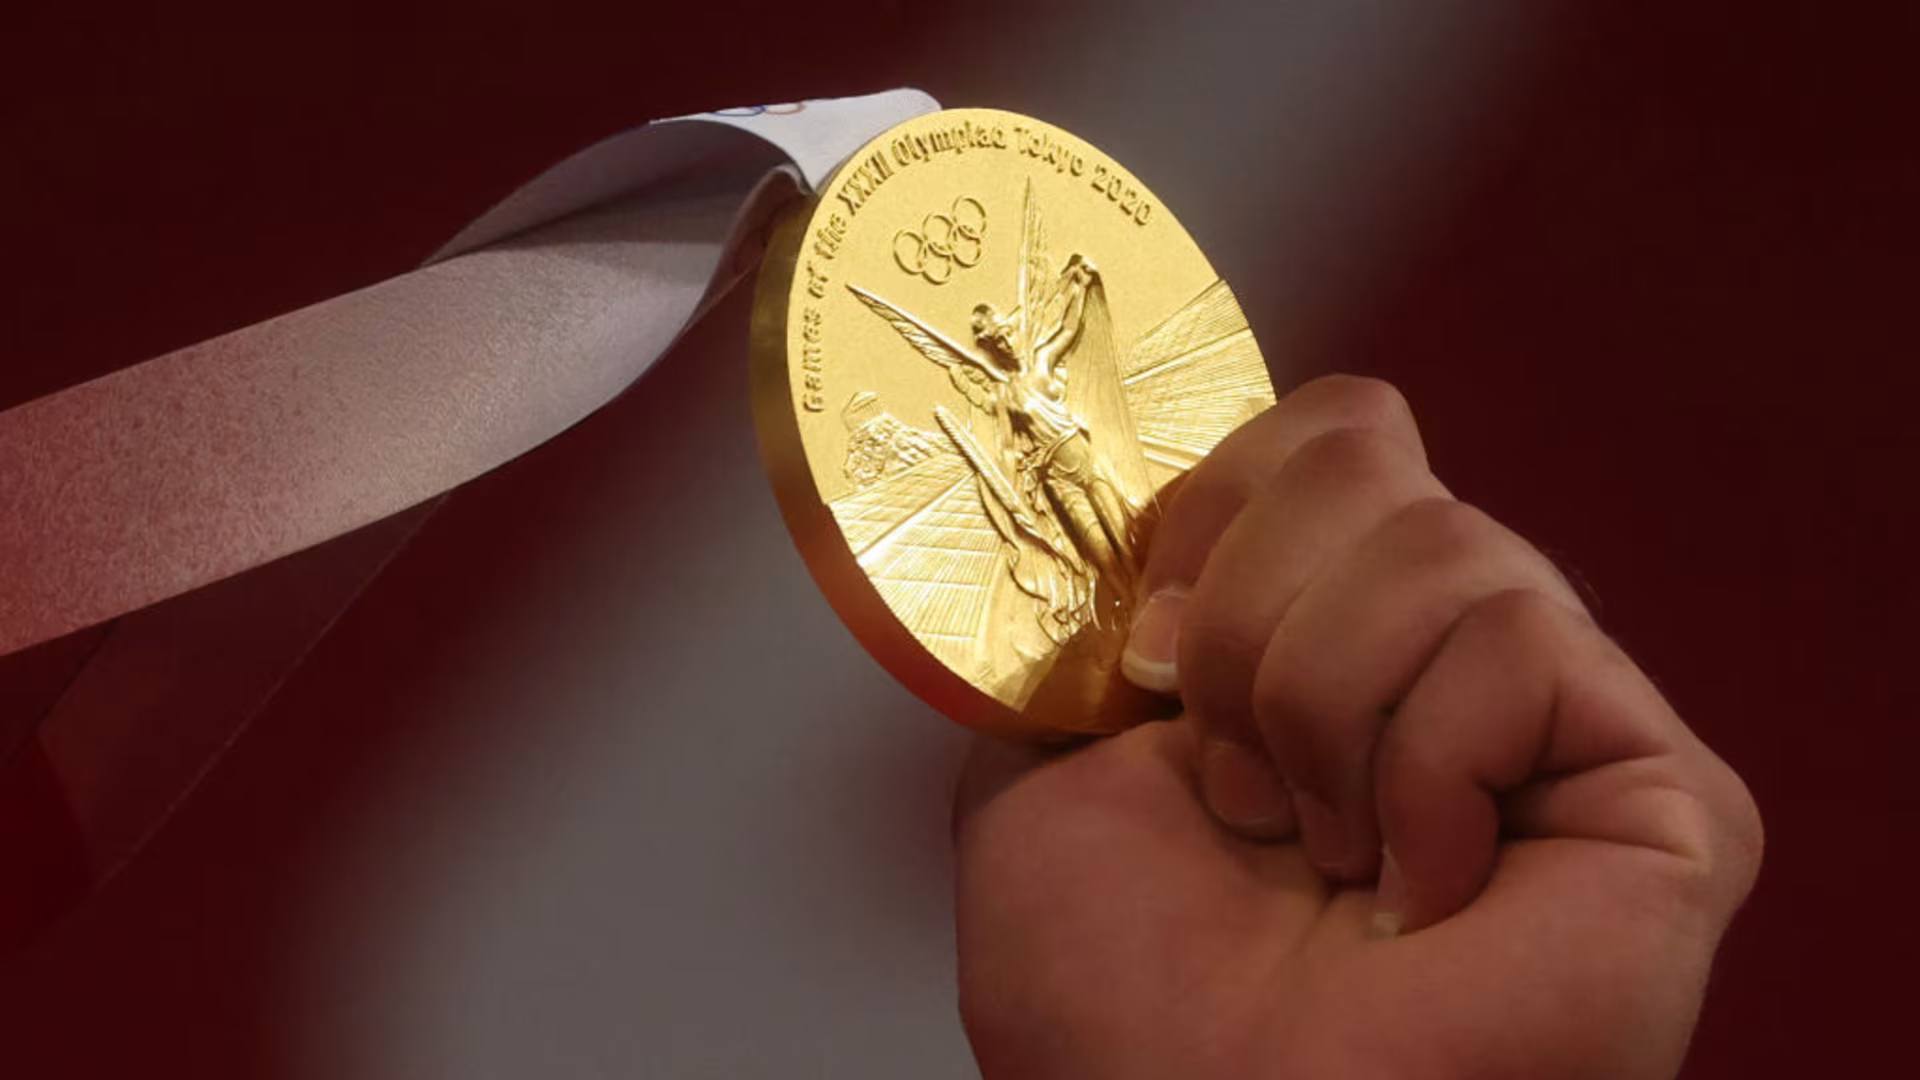
\includegraphics[width=0.7\linewidth]{fig/background}
		\caption{The medals of the 2024 Paris Olympics}
	\end{figure}
	
	\subsection{Restatement and Analysis of the Problem}
	Based on the provided historical data-set of the Olympic Games from 1896 to 2024, we are employed to analyze and answer the following questions:
	\begin{enumerate}
		\item 
		Develop a \textbf{prediction model} to forecast the number of medals each country will win in 2028, and identify countries that may progress or regress. 
		\item 
		Provide \textbf{prediction intervals} and estimates of \textbf{uncertainty} and metrics to measure the model's performance.
		\item 
		Estimate the number of countries that will win their \textbf{first medal} and the probability of this happening.
		\item 
		Analyze the \textbf{relationship} between specific Olympic events (in terms of quantity and type) and the number of medals, explore which events are more important, and the impact of the host country's event selection strategy on the outcome.
		\item 
		Verify whether the \textbf{mobility of coaches} significantly enhances a country's performance in specific sports (such as Lang Ping and Bela Karolyi).
		\item 
		Quantify the contribution of\textbf{ coaching effectiveness} to the number of medals, and recommend key sports for investment and expected returns for the three countries.
		\item 
		Extract the less-attended-to patterns from the model and provide strategic \textbf{suggestions} for the Olympic Committee.
	\end{enumerate}
	
	
	
	%对于Task1,我们选取7个指标,建立了基于LSTM的奖牌数量预测模型,并使用贝叶斯估计给出了区间预测,而对于从未获奖的国家,我们根据新增的event、运动员数量、历史参与趋势,建立了基于SVM的“首奖突破”预测模型。
	%对于Task2,我们分析了“伟大教练”效应的影响。
	
	
	
	
	
	
	
	
	
	\subsection{Overview of Our Work}
		\begin{figure}[H]
		\centering
		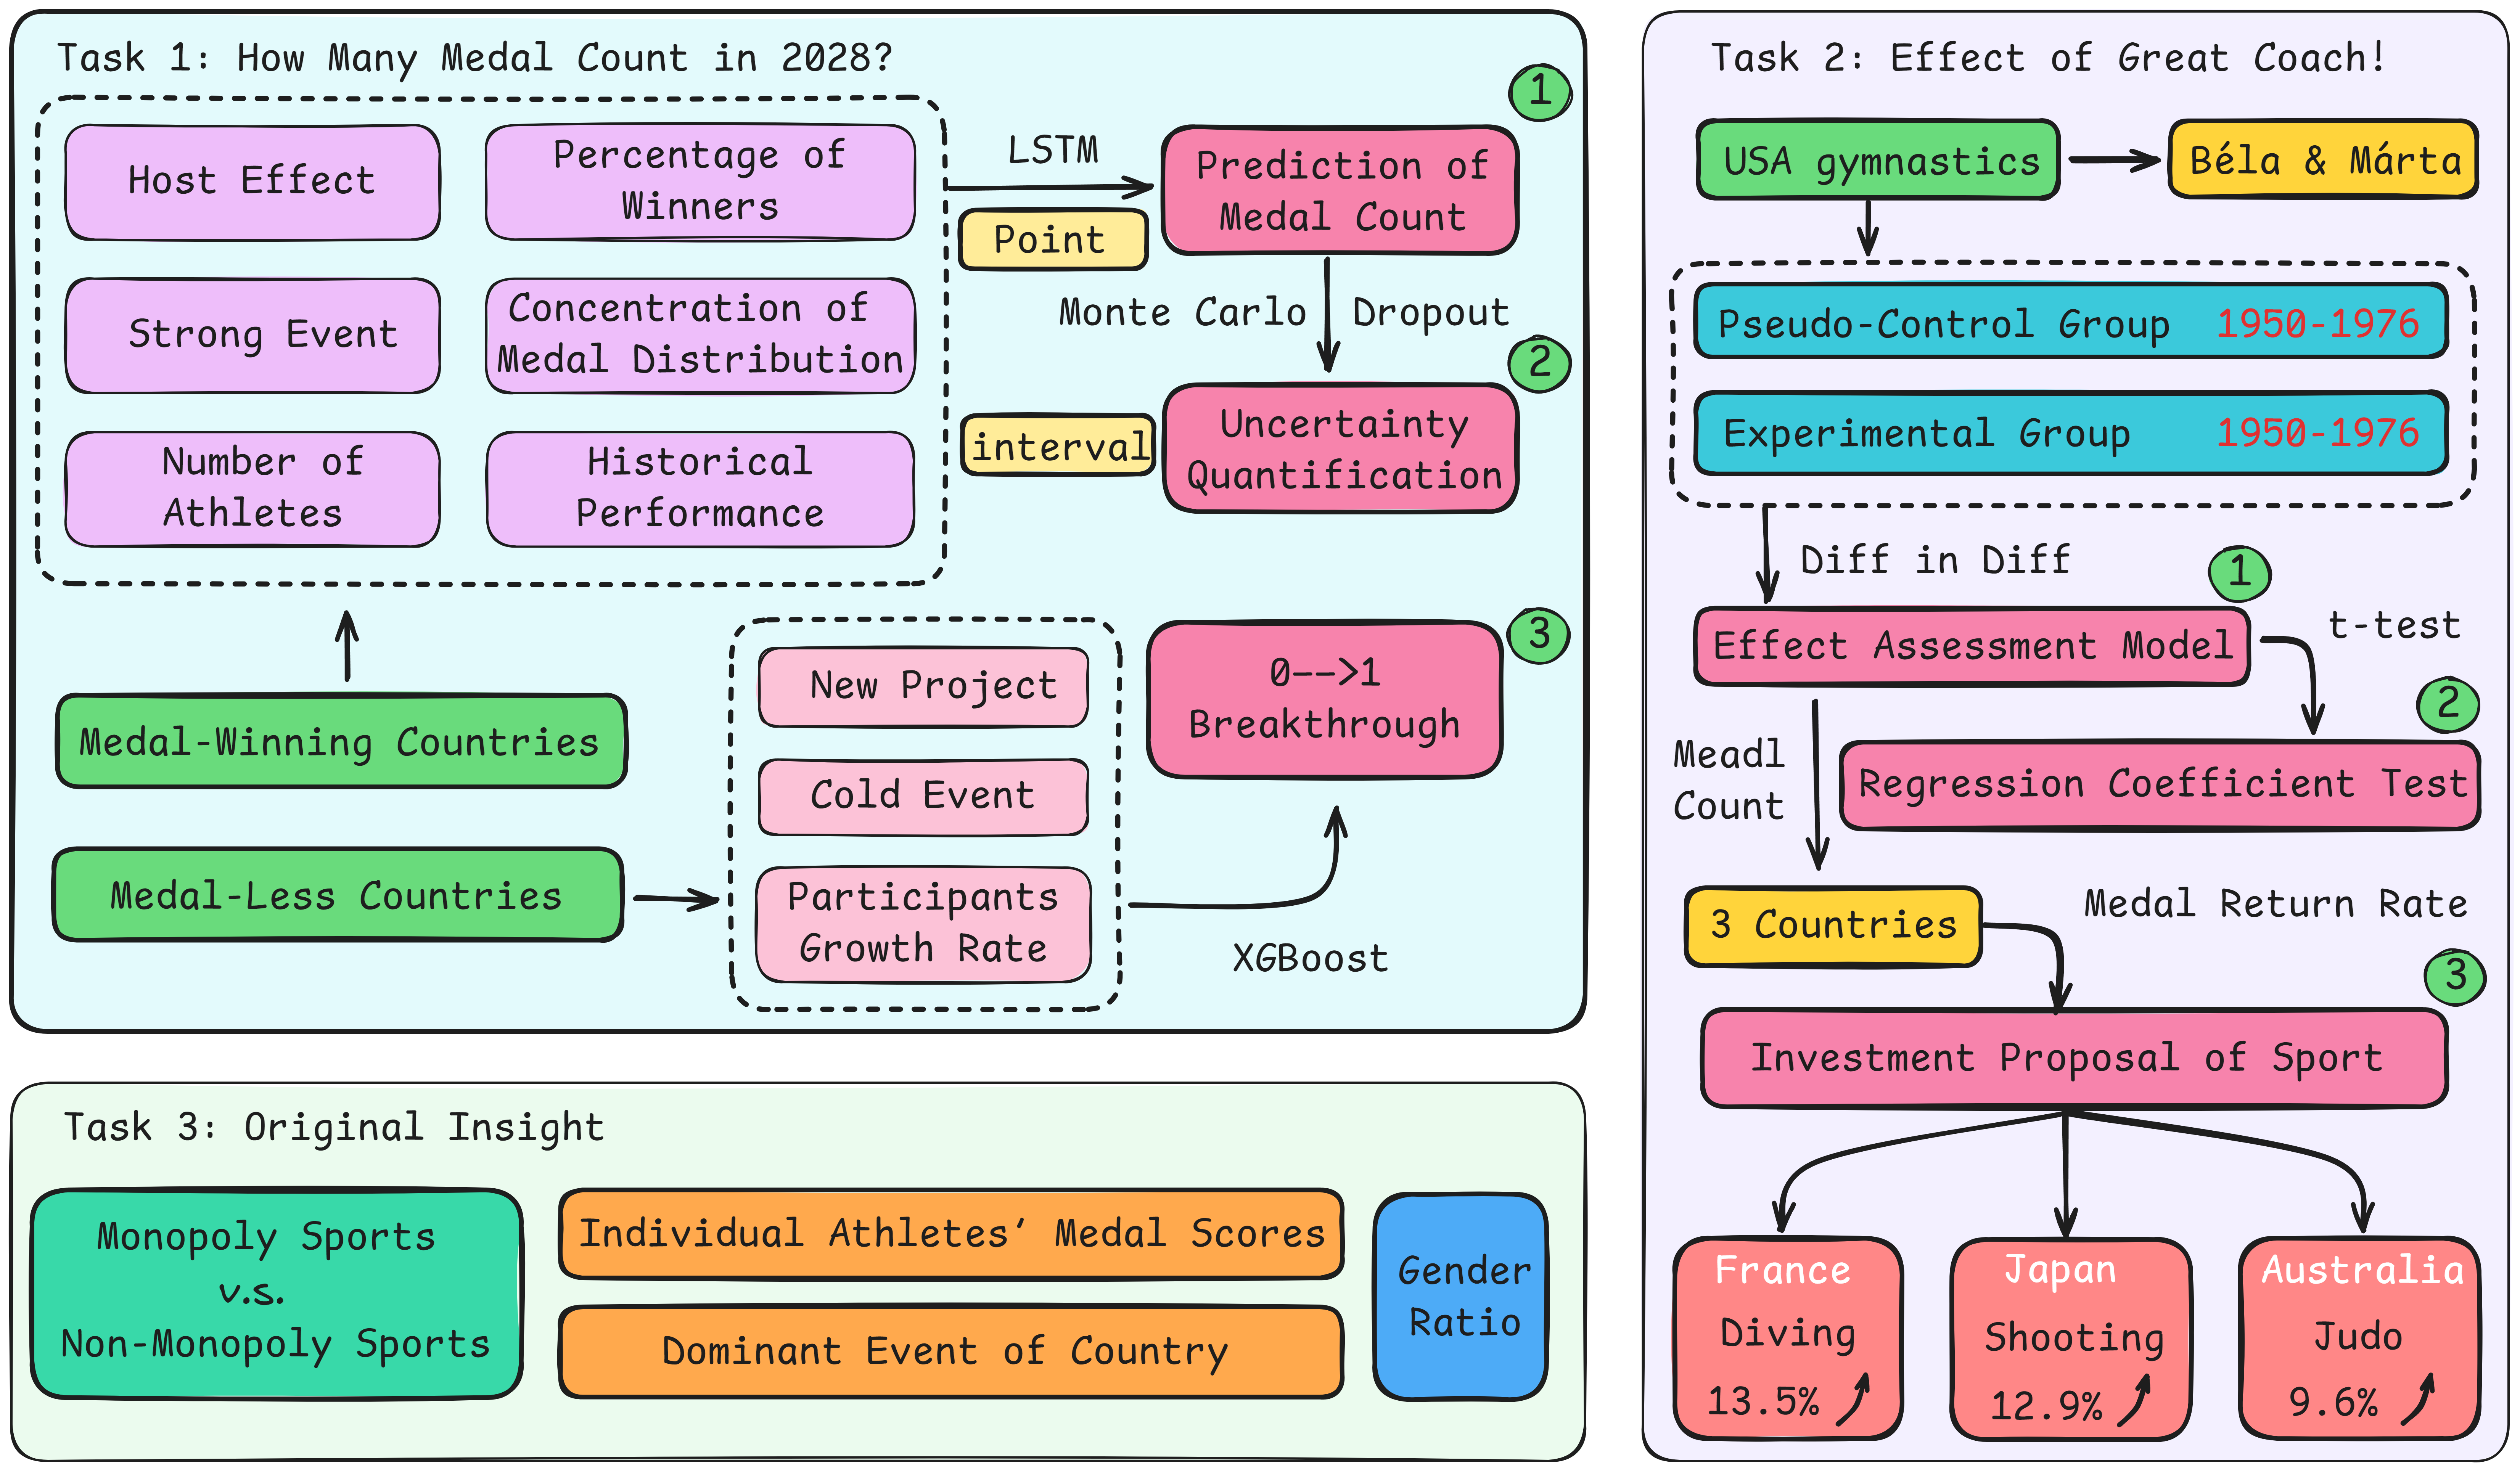
\includegraphics[width=1\linewidth]{fig/OurWork.png}
		\caption{Overview of Our Work}
		\label{fig:Overview of Our Work}
	\end{figure}
	%\begin{itemize}
	%	\item {\bf 111}. ...
	%	\item {\bf 222}. ...
	%	
	%	\begin{itemize}
		%		\item[1)] ... 
		%		\item[2)] ...
		%		\item[3)] ...
		%		\item[4)] ...
		%	\end{itemize}
	%	
	%\end{itemize}
	
	
	
	
	
	
	
	
	%%%%%%%%%%%%%%%%%%%%%%%%%%%%%%%%%%%%%%%%
	%%%%%%%%%%%%%%%%% 模型假设 %%%%%%%%%%%%%%%%%
	%%%%%%%%%%%%%%%%%%%%%%%%%%%%%%%%%%%%%%%%
\section{Assumptions and Justification}

\begin{enumerate}[leftmargin=0.15in, labelsep=0.1in, itemsep=10pt, parsep=5pt]
	\item \textbf{Historical medal data exhibits temporal dependencies that reflect future medal trends. }
	
	This suggests that historical performance can offer insights into future outcomes, and thus, should be treated as a time series when making predictions.
	
	\item \textbf{Monte Carlo Dropout approximates Bayesian inference by quantifying prediction uncertainty through multiple stochastic samplings.}
	
	This technique provides a robust mechanism for estimating confidence intervals and is useful in scenarios with incomplete or noisy data.
	
	\item \textbf{Historical data distributions of non-medal-winning countries align with those of future potential medal-winning nations.} 
	
	This assumption supports the idea that non-medal-winning countries have similar characteristics to those that may perform well in future Olympics, making them a valuable reference for predicting future medal potential.
	
	\item \textbf{The impact of coaching remains independent of confounding variables (e.g., athlete training conditions, changes in international competition rules).} 
	
	This assumption isolates the effect of coaching from other factors that might influence performance, ensuring that coaching effects can be accurately assessed.
\end{enumerate}

	%%%%%%%%%%%%%%%%%%%%%%%%%%%%%%%%%%%%%%%%
	%%%%%%%%%%%%%%%%% 符号说明 %%%%%%%%%%%%%%%%%
	%%%%%%%%%%%%%%%%%%%%%%%%%%%%%%%%%%%%%%%%
\section{List of Notations}
\begin{center}
	\begin{tabular}{ll}
		\toprule
		{\bf Symbols} & {\bf Description}  \\
		\midrule 
		$A_{C},A_{S}$ & Set of country, all sports in Olympic.\\
		$A_{T}$ & $\{1,\dots,30\}$, representing the ordinal number of year Olympic held. \\
		$A_E(j)$ & Represents the set of events inside the sport j.\\
		$A_{H}(t)$ & Set of host country in year $t$. \\
		$MG_{t,i,j,k}$ & Number of gold medals country $i$ won in sport $j$ at event $k$ in year t. \\
		$MS_{t,i,j,k}$ & Number of silver medals country $i$ won in sport $j$ at event $k$ in year t. \\
		$MB_{t,i,j,k}$ & Number of bronze medals country $i$ won in sport $j$ at event $k$ in year t. \\
		$MT_{t,i}$ & Number of total medals country $i$ won in year $t$. \\
		$N_{athletes}(t,i)$ & Total number of athletes from country $i$ in year $t$. \\
		$N_{award}(t,i)$ & Number of athletes who won medals from country $i$ in year $t$. \\
		$H(t,i)$ & Host effect. \\
		$G_{\text{growth}}(t,i)$ & Growth rate of the number of athletes from country $i$ in year $t$.\\
		$P_{Medal}(t,i)$ & Probability of country $i$ winning a medal in year $t$.\\
		$P_{Gold}(t,i)$ & Probability of country $i$ winning a gold medal in year $t$.\\
		\bottomrule
	\end{tabular}
\end{center}

\noindent Note: The Summer Olympics have been held for a total of 32 sessions.
	
	
	
	
	
	
	
	
	

	
	
	
	
	
	
	%%%%%%%%%%%%%%%%%%%%%%%%%%%%%%%%%%%%%%%%
	%%%%%%%%%%%%%%%%% 文献条目 %%%%%%%%%%%%%%%%%
	%%%%%%%%%%%%%%%%%%%%%%%%%%%%%%%%%%%%%%%%
	\newpage
	\addcontentsline{toc}{section}{References} % 手动添加到目录
	\printbibliography
	
	
	
	
	%%%%%%%%%%%%%%%%%%%%%%%%%%%%%%%%%%%%%%%%
	%%%%%%%%%%%%%%%%% 附录 %%%%%%%%%%%%%%%%%
	%%%%%%%%%%%%%%%%%%%%%%%%%%%%%%%%%%%%%%%%
	\begin{appendices}
		\section{First appendix}
		\section{Second appendix}
	\end{appendices}
	
	
	
	
	%%%%%%%%%%%%%%%%%%%%%%%%%%%%%%%%%%%%%%%%
	%%%%%%%%%%%%%%%%% AI使用 %%%%%%%%%%%%%%%%%
	%%%%%%%%%%%%%%%%%%%%%%%%%%%%%%%%%%%%%%%%
	\newpage
	\newcounter{lastpage}
	\setcounter{lastpage}{\value{page}}
	\thispagestyle{empty} 
	
	\section*{Report on Use of AI}
	
	\begin{enumerate}
		\item OpenAI ChatGPT (Nov 5, 2023 version, ChatGPT-4,) 
		\begin{description}
			\item[Query1:] <insert the exact wording you input into the AI tool> 
			\item[Output:] <insert the complete output from the AI tool>
		\end{description}
		
		\item OpenAI ChatGPT (Nov 5, 2023 version, ChatGPT-4,) 
		\begin{description}
			\item[Query1:] <insert the exact wording you input into the AI tool> 
			\item[Output:] <insert the complete output from the AI tool>
		\end{description}
		
	\end{enumerate}
	
	% 重置页码
	\clearpage
	\setcounter{page}{\value{lastpage}}
	
	
	
	
	
	
\end{document}